\chapter{РЕЗУЛЬТАТЫ ВЫПОЛНЕНИЯ РАБОТЫ}
\label{ch:Results}

В результате выполнения работы, нами были получены профили скорости (т.е. зависимость параметра порядка от высоты) для течения Куэтта идеальной самодвижущейся жидкости по модели Vicsek'a.

\begin{figure}
    \centering
        \begin{subfigure}{\textwidth}
        \centering
            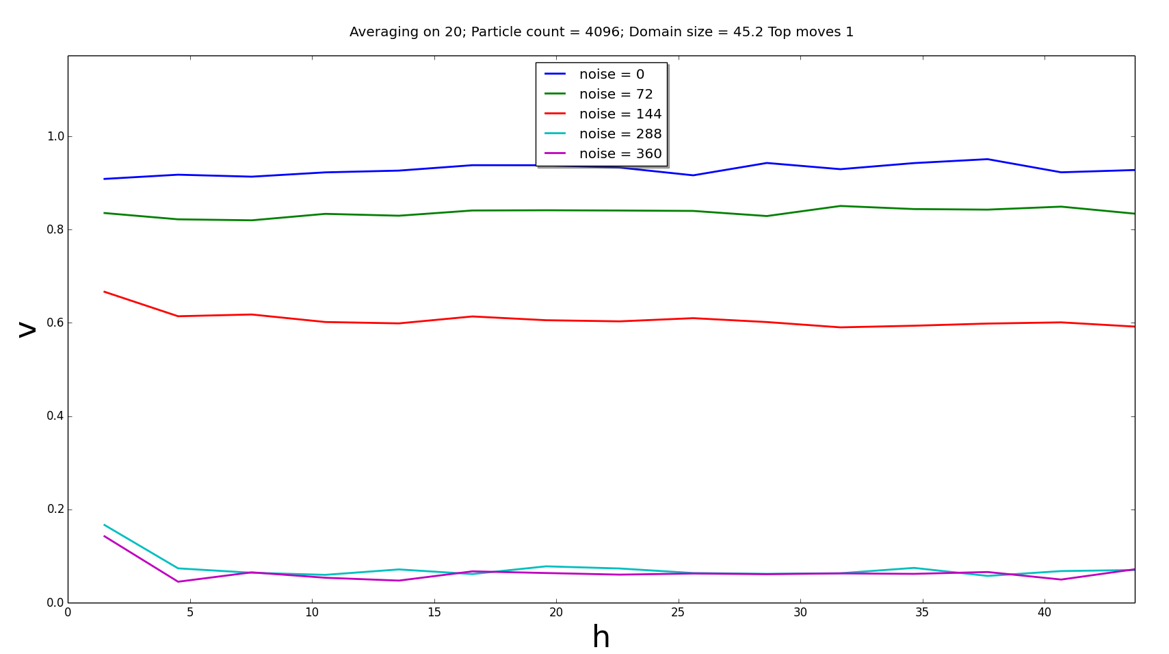
\includegraphics[height=0.3\textheight]{Images/4k_x20}
            \caption{Число частиц: 4096; Плотность: 2; Число конфигураций: 20; Зеркальная граница}
            \label{fig:Results:32k}
        \end{subfigure}
        \begin{subfigure}{\textwidth}
        \centering
            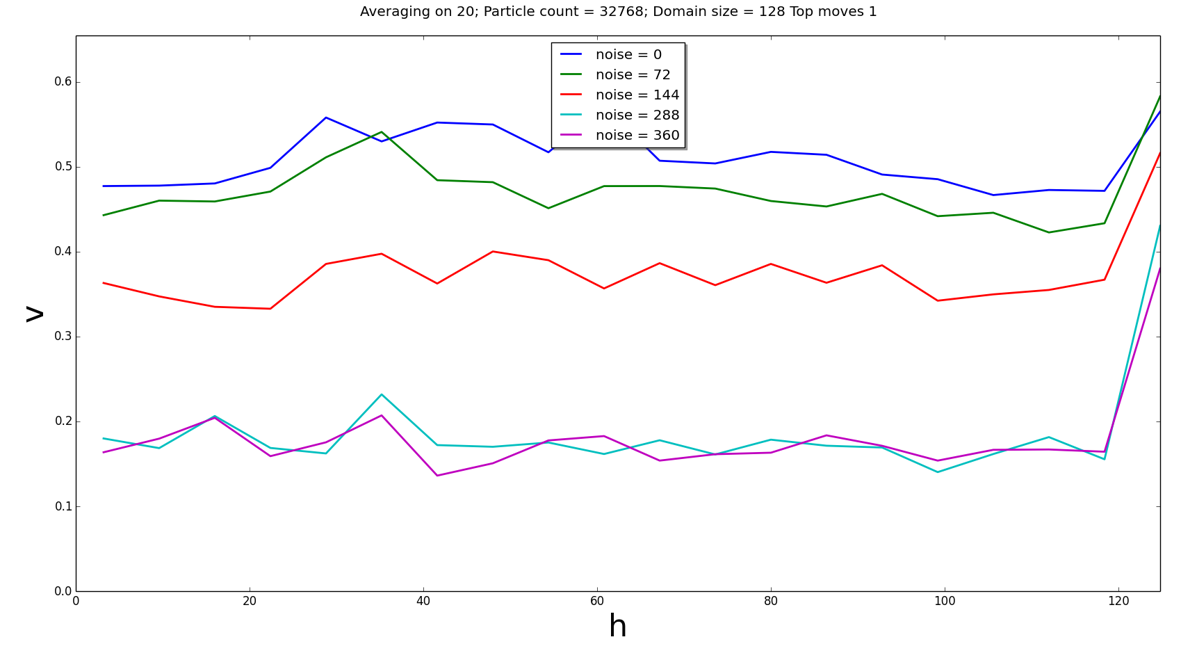
\includegraphics[height=0.3\textheight]{Images/32k_x20}
            \caption{Число частиц: 32768; Плотность: 2; Число конфигураций: 20; Зеркальная граница}
            \label{fig:Results:32kOld}
        \end{subfigure}
        \begin{subfigure}{\textwidth}
        \centering
            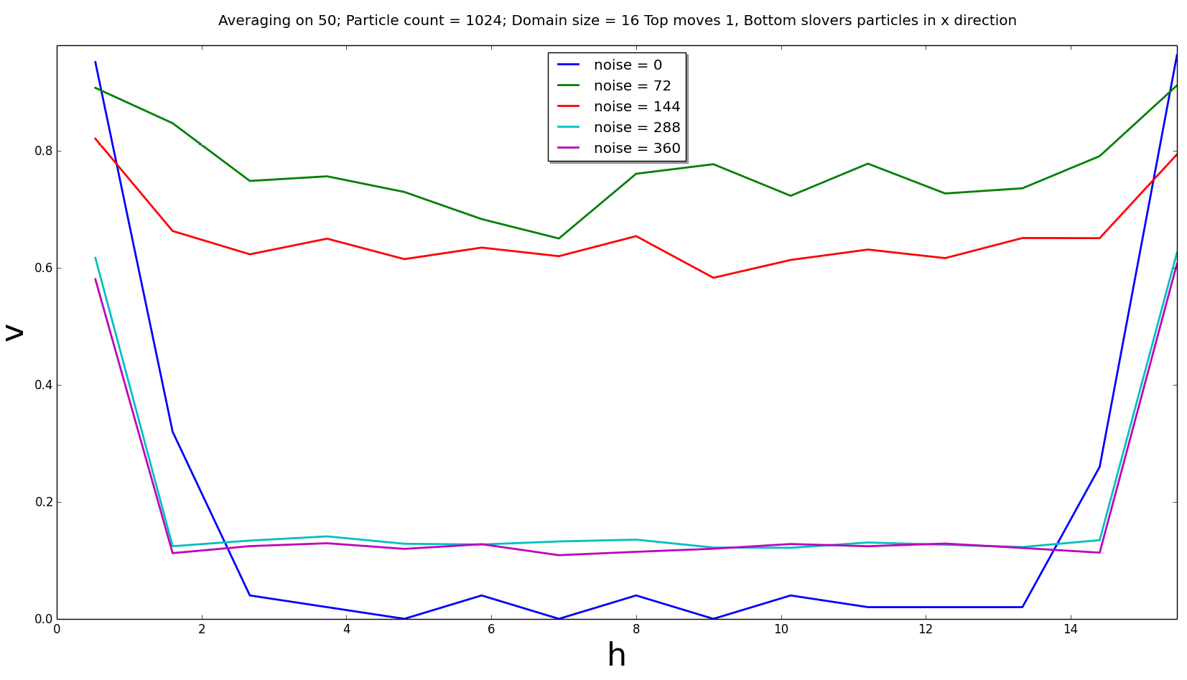
\includegraphics[height=0.3\textheight]{Images/1k_x50_NotMirror}
            \caption{Число частиц: 1024; Плотность: 4; Число конфигураций: 50; Шероховатая граница}
            \label{fig:Results:4kNew}
        \end{subfigure}
    \caption{Зависимость параметра порядка от высоты для течения Куэтта при разных значениях шума.}
    \label{fig:Results}
\end{figure}

Предложенный алгоритм определения стабилизации состояния системы оправдал себя. Поскольку определение времени стабилизации не входило в тему данной работы, то специальных замеров не проводилось, но среднее значение времени симуляции для каждого значения шума составило $10^{2-3}$ по порядку величины, увеличиваясь с увеличением количества частиц.

\begin{figure}
    \centering
        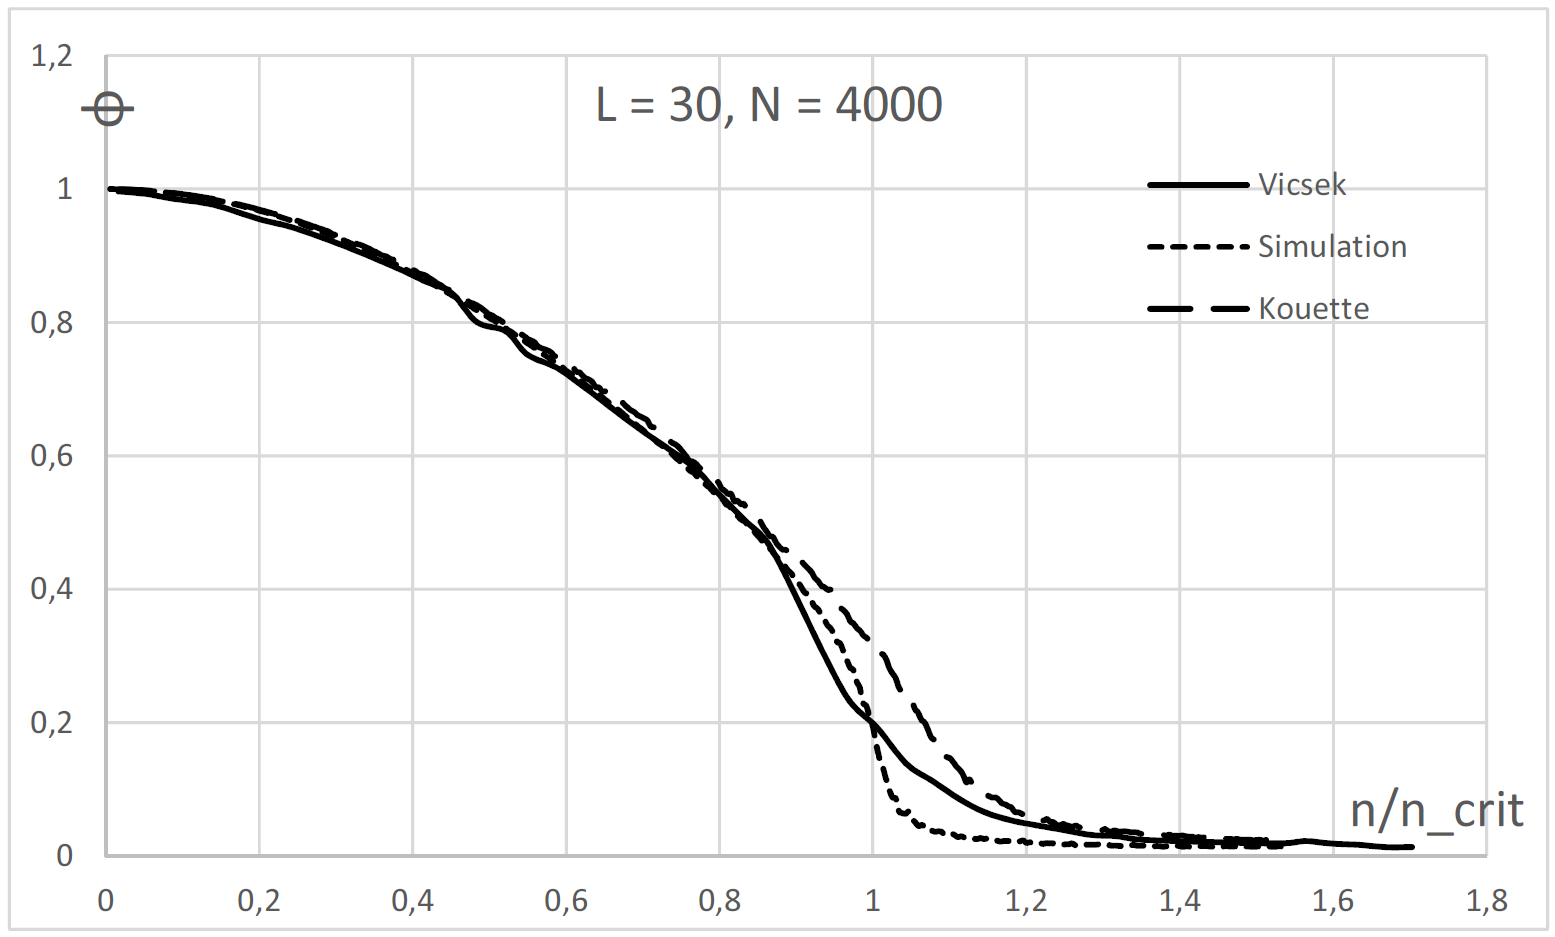
\includegraphics[height=0.33\textheight]{Images/CheckerResult}
    \caption{Зависимость параметра порядка от безразмерного шума}
    \label{fig:CheckerResults}
\end{figure}

Проверка работоспособности алгоритма, и его невлияние на предполагаемый результат была проведена прямой симуляцией системы, аналогичной одной из \cite{vicsek1995}, и были построены графики зависимости параметра порядка от безразмерного шума, представленные на рис. \ref{fig:CheckerResults}

Кроме того, были проведены более длительные симуляции для отдельных значений шума (в частности, очень большого и очень низкого). Полученные результаты не вошли в эту работу по причине того, что они аналогичны представленным на рис. \ref{fig:Results}.

Побочным результатом выполнения работы также стало создание программы, способной выполнять симуляции идеальной самодвижущейся жидкости по модели Vicsek'a на GPU, и легко доступной для модернизации.

\likechapter{ВЫВОДЫ}
\label{ch:Conclusion}
Главным выводом, который можно сделать из результатов работы, является полная несостоятельность теоретического описания, основанного на подходе Больцмана, и дающего в результате ненулевые значения вязкости, поскольку, как видно из представленных результатов, профили скорости в случае идеальной самодвижущейся жидкости никак не соответствуют предполагаемым профилям Куэттовсого потока.

Благодаря предложенному алгоритму удалось радикально сократить время, необходимое для проведения симуляций. Конечно, по мере стремления к термодинамическому пределу требуемое для релаксации время будет увеличиваться, но для всех разумных значений числа частиц алгоритм может быть полезен, если правильно выбрать параметр стабилизации.

Наконец, использование GPU для проведения физических рассчетов с высоким фактором параллелизации не только оправдано, но и необходимо - замеренная производительность GPU превышает производительность CPU более чем в 100 раз!